% ============================================================================
%  অধ্যায় ৫ — ইউক্লিডীয় জ্যামিতি ১
%  COMPILE WITH XeLaTeX  (twice, so the point total resolves)
%  Overleaf: Menu -> Compiler -> XeLaTeX
% ============================================================================
\documentclass[11pt]{article}
\usepackage{bnhandout}          % add [nosol] for a student edition
\usepackage{tikz}               % harmless if bnhandout already loads it

\hauthor[https://jugantordey.github.io/]{Jugantor Dey}
\hseries{\textit{Mathematics for the Physics Olympiad}}

\begin{document}

\handouttitle{Chapter 5 : Euclidean Geometry I}

\noindent
এই অধ্যায়ের একমাত্র পূর্বশর্ত অধ্যায় ১। সেখান থেকে যা লাগবে তা হলো
প্রমাণের অভ্যাস; বিশেষ করে অসম্ভব কিছু ধরে নিয়ে বিরোধে পৌঁছানো, আর একটিমাত্র
counterexample দিয়ে দাবি ভেঙে ফেলা। অধ্যায় ২-এর সরল সমীকরণ দু-একটা সমস্যায়
কাজে লাগবে, তার বেশি কিছু নয়।

জ্যামিতি এই সিরিজে ঢুকছে দুটো কারণে, আর কোনোটাই ``পরীক্ষায় আসে'' নয়। প্রথমত,
এটাই প্রথম জায়গা যেখানে গণিত একটা \emph{কাঠামো} হিসেবে দাঁড়ায় : অল্প কয়েকটা
মেনে নেওয়া কথা থেকে শুরু করে বাকি সব কিছু প্রমাণ করে বের করা। এই অভ্যাসটাই
পদার্থবিজ্ঞানের গোটা পদ্ধতি। দ্বিতীয়ত, এখানে যে ছবিগুলো আঁকতে শিখবে, সেগুলোই
পরে বল-চিত্র, আলোর পথ আর vector-এর ছবি হয়ে ফিরে আসবে।

সতর্কতা: এই অধ্যায়ে ছবি আছে, কিন্তু ছবি কোনো প্রমাণ নয়। ছবি দেখে কোনো কথা
সত্য মনে হলেই সেটা সত্য হয়ে যায় না। ছবি কেবল বলে দেয় কী প্রমাণ করতে হবে।
এখানে মোট \totalpoints\ পয়েন্ট আছে।

\section{বিন্দু, রেখা, কোণ}

\begin{idea}[সংজ্ঞা একটা চুক্তি]
গণিতে সংজ্ঞা কোনো বর্ণনা নয়, একটা চুক্তি। ``সমদ্বিবাহু ত্রিভুজ মানে যার দুটি
বাহু সমান'' --- এই বাক্যটা ত্রিভুজ সম্পর্কে কোনো তথ্য দিচ্ছে না, বরং একটা শব্দের
ব্যবহার বেঁধে দিচ্ছে। চুক্তিটা মেনে নেওয়ার পর ``এই ত্রিভুজটা সমদ্বিবাহু কি না''
প্রশ্নের উত্তর মতামতের বিষয় নয়; দুটি বাহু সমান কি না, কেবল সেটাই দেখার বিষয়।

এর একটা সরাসরি ফল আছে, যা শুরুর দিকে অস্বস্তিকর লাগে: সব শব্দের সংজ্ঞা দেওয়া
সম্ভব নয়। ``রেখা'' সংজ্ঞায়িত করতে গেলে অন্য শব্দ লাগবে, তার জন্য আরও শব্দ ---
এভাবে অসীমকাল চলবে, নয়তো ঘুরে এসে নিজের লেজ কামড়াবে। তাই কয়েকটা শব্দ
\emph{অসংজ্ঞায়িত} রেখে দিতে হয়। আমরা রাখছি তিনটি: বিন্দু, রেখা, তল।
\end{idea}

\begin{idea}[যা আমরা প্রমাণ ছাড়াই মেনে নিচ্ছি]
অসংজ্ঞায়িত শব্দ নিয়ে কাজ করতে হলে কিছু কথা প্রমাণ ছাড়াই মেনে নিতে হয়। এদের বলে
স্বীকার্য (axiom)। এই অধ্যায়ে আমরা যা যা মেনে নিচ্ছি, তার পুরো তালিকা এখানে। এর বাইরে আর কিছু ধার করা হবে না, আর যা কিছু ব্যবহার করা হবে তা হয় এই তালিকায়
থাকবে, নয়তো প্রমাণ করা হবে। নিচের প্রতিটি স্বীকার্য পড়ার সময় খাতায় একটা রাফ চিত্র এঁকে ব্যাপারটা বোঝার চেষ্টা করো এবং চিন্তা করো যে স্বীকার্যগুলোকে আসলে কেন সত্য বলে মেনে নেওয়া হচ্ছে। আরো ভালো হয় যদি এই পুরো কাজটা কোনো খাতা-কলম ছাড়াই নিজের চিন্তার জগতে কল্পনা করতে পারো!
\begin{enumerate}
  \item দুটি ভিন্ন বিন্দুর মধ্য দিয়ে একটি এবং কেবল একটি সরলরেখা যায়।
  \item কোণ ডিগ্রিতে মাপা যায়; সন্নিহিত কোণের পরিমাপ যোগ হয়; সরলকোণ $180^\circ$।
  \item সমান্তরাল স্বীকার্য: কোনো রেখার বাইরের একটি বিন্দু দিয়ে সেই রেখার
        সমান্তরাল ঠিক একটি রেখা আঁকা যায়।
  \item একটি ছেদক দুটি সমান্তরাল রেখাকে ছেদ করলে অনুরূপ কোণগুলো সমান, এবং এর
        বিপরীতটাও সত্য।
  \item সর্বসমতার শর্ত SSS, SAS, ASA।
  \item সদৃশতার শর্ত AA, SAS, SSS। (ঙ আর চ এখন না বুঝলেও সমস্যা নেই, পরবর্তীতে এর প্রয়োগ দেখলেই বুঝতে পারবে।)
  \item আয়তক্ষেত্রের ক্ষেত্রফল $=$ দৈর্ঘ্য $\times$ প্রস্থ; সর্বসম চিত্রের
        ক্ষেত্রফল সমান; দুটি ক্ষেত্রফল সরাসরি যোগ করা যায়।
  \item প্রতিটি অঋণাত্মক সংখ্যার একটিমাত্র অঋণাত্মক বর্গমূল আছে।
\end{enumerate}
\end{idea}

\noindent
এবার কয়েকটা সংজ্ঞা। দুটি বিন্দু $A$ ও $B$ নিলে তাদের মধ্যবর্তী অংশসহ দুই প্রান্ত
মিলে হয় রেখাংশ $\overline{AB}$; তার দৈর্ঘ্য লিখি $AB$। একটি বিন্দু থেকে শুরু করে
এক দিকে অসীম পর্যন্ত গেলে হয় রশ্মি। একই প্রান্তবিন্দু থেকে বেরোনো দুটি রশ্মি
মিলে তৈরি করে কোণ; $O$ শীর্ষবিন্দু হলে লিখি $\angle AOB$।

\begin{example}
$O$ বিন্দু থেকে তিনটি রশ্মি $OA$, $OB$, $OC$ বেরিয়েছে, যেখানে $OB$ রশ্মিটি
$\angle AOC$-এর ভেতরে। যদি $\angle AOB = 35^\circ$ এবং $\angle BOC = 48^\circ$
হয়, তবে $\angle AOC$ কত? আর $\angle AOC$-এর প্রবৃদ্ধ কোণটি কত?
\end{example}

\begin{solbox}
$OB$ যেহেতু ভেতরে, স্বীকার্য ২ অনুযায়ী কোণ দুটি যোগ হয়:
\[
  \angle AOC = 35^\circ + 48^\circ = 83^\circ .
\]
একই দুটি রশ্মি কিন্তু দুটি কোণ ঘেরে --- ভেতরেরটা $83^\circ$, আর বাইরেরটা বাকি
অংশ:
\[
  360^\circ - 83^\circ = 277^\circ .
\]
এটাই প্রবৃদ্ধ কোণ (reflex angle)। লক্ষ করো, ``$\angle AOC$'' লেখাটা আসলে
দ্ব্যর্থক --- দুটো কোণের যেকোনোটাই বোঝাতে পারে। রীতি অনুযায়ী আমরা ছোটটাই বুঝি,
কিন্তু সেটা একটা \emph{চুক্তি}, আবিষ্কৃত সত্য নয়। প্রবৃদ্ধ কোণ বোঝাতে চাইলে
আলাদা করে বলে দিতে হবে।
\end{solbox}

\prob{2} স্বীকার্য ১ ব্যবহার করে প্রমাণ করো যে দুটি ভিন্ন সরলরেখা একের বেশি
বিন্দুতে ছেদ করতে পারে না।

\begin{sol}
বিরোধ ধরে এগোই। ধরি $\ell$ ও $m$ দুটি ভিন্ন সরলরেখা, এবং তারা দুটি ভিন্ন বিন্দু
$P$ ও $Q$-তে ছেদ করেছে।

তাহলে $\ell$ রেখাটি $P$ ও $Q$ দুটোর মধ্য দিয়েই যায়, এবং $m$ রেখাটিও $P$ ও $Q$
দুটোর মধ্য দিয়েই যায়। কিন্তু স্বীকার্য ১ বলছে দুটি ভিন্ন বিন্দুর মধ্য দিয়ে
\emph{কেবল একটি} সরলরেখা যায়। সুতরাং $\ell$ ও $m$ একই রেখা; যা আমাদের ধরে
নেওয়া কথার (রেখাদ্বর ভিন্ন) বিরোধী।

তাই ছেদবিন্দু দুটি হতে পারে না। সর্বাধিক একটি।

লক্ষ করো, ``অন্তত একটি ছেদবিন্দু থাকে'' প্রমাণ হয়নি এবং হওয়ার কথাও নয় : সমান্তরাল রেখারা
মোটেও ছেদ করে না।
\end{sol}

\section{কোণের শ্রেণিবিভাগ}

\noindent
পরিমাপ অনুযায়ী কোণের নামগুলো নিছক চুক্তি, তাই এক নজরে সেরে নিই। $0^\circ$ ও
$90^\circ$-এর মাঝে হলে সূক্ষ্মকোণ; ঠিক $90^\circ$ হলে সমকোণ; $90^\circ$ ও
$180^\circ$-এর মাঝে হলে স্থূলকোণ; ঠিক $180^\circ$ হলে সরলকোণ; $180^\circ$ ও
$360^\circ$-এর মাঝে হলে প্রবৃদ্ধ কোণ; ঠিক $360^\circ$ হলে পূর্ণকোণ।

দুটি কোণের সমষ্টি $90^\circ$ হলে তারা পরস্পর পূরক (complementary), আর
$180^\circ$ হলে পরস্পর সম্পূরক (supplementary)। শব্দ দুটি গুলিয়ে ফেলা খুব সাধারণ; তবে মনে রাখার সহজ উপায় আছে : পূরক আর সম্পূরক এর সাথে $90^\circ$ আর $180^\circ$ এর সম্পর্ক আছে এটা তো মনে থাকবেই। এখন "পূরক" কথাটা যেহেতু "সম্পূরক" কথাটা থেকে ছোট, তাই পূরকের সাথে সম্পর্ক $90^\circ$-এর, যা $180^\circ$ থেকে ছোট।

\begin{idea}[বিপ্রতীপ কোণ সমান]
দুটি সরলরেখা ছেদ করলে যে চারটি কোণ তৈরি হয়, তার মধ্যে মুখোমুখি জোড়াগুলোকে বলে
বিপ্রতীপ কোণ (vertically opposite angles)। এরা সবসময় সমান, আর এটা প্রমাণ করা যায়।

ধরি ছেদবিন্দুতে পরপর চারটি কোণ $w, x, y, z$। $w$ ও $x$ একসাথে একটা সরলকোণ গড়ে,
তাই $w + x = 180^\circ$। আবার $x$ ও $y$ও একসাথে সরলকোণ গড়ে, তাই
$x + y = 180^\circ$। দুটো মিলিয়ে
\[
  w + x = x + y \implies w = y .
\]
একই যুক্তিতে $x = z$। প্রমাণে কোথাও ছবির উপর ভরসা করতে হয়নি, কেবল স্বীকার্য ২
লেগেছে।
\end{idea}

\begin{idea}[ছেদক ও সমান্তরাল রেখা]
নিচের ছবিতে $\ell_1 \parallel \ell_2$ এবং $t$ হলো ছেদক (secant)।

\begin{center}
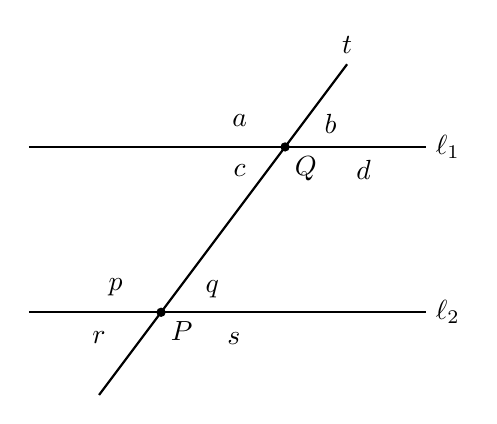
\begin{tikzpicture}[scale=1.05]
  \draw[thick] (-1.6,2)--(3.2,2) node[right]{$\ell_1$};
  \draw[thick] (-1.6,0)--(3.2,0) node[right]{$\ell_2$};
  \draw[thick] (-0.75,-1.0)--(2.25,3.0) node[above]{$t$};
  \fill (1.5,2) circle (1.6pt) node[below right]{$Q$};
  \fill (0,0) circle (1.6pt) node[below right]{$P$};
  \node at (0.95,2.32) {$a$};
  \node at (2.05,2.28) {$b$};
  \node at (0.95,1.72) {$c$};
  \node at (2.45,1.72) {$d$};
  \node at (-0.55,0.30) {$p$};
  \node at (0.62,0.28) {$q$};
  \node at (-0.75,-0.30) {$r$};
  \node at (0.88,-0.32) {$s$};
\end{tikzpicture}
\end{center}

\noindent
দুই রেখার \emph{মাঝের} কোণগুলোকে বলে অন্তঃস্থ কোণ --- এখানে $c, d, p, q$।

\textbf{অনুরূপ কোণ} (corresponding): একই দিকে, একই অবস্থানে --- $a$ ও $p$,
$b$ ও $q$, $c$ ও $r$, $d$ ও $s$। স্বীকার্য ৪ অনুযায়ী এরা সমান।

\textbf{একান্তর কোণ} (alternate interior): অন্তঃস্থ, কিন্তু $t$-এর দুই পাশে ---
$c$ ও $q$, এবং $d$ ও $p$। এরাও সমান, আর এটা প্রমাণ করা যায়: $c = b$ (বিপ্রতীপ)
এবং $b = q$ (অনুরূপ), সুতরাং $c = q$।

\textbf{একই পাশের অন্তঃস্থ কোণ} (co-interior): অন্তঃস্থ, $t$-এর একই পাশে ---
$c$ ও $p$, এবং $d$ ও $q$। এদের সমষ্টি $180^\circ$: $p + q = 180^\circ$ (সরলকোণ)
এবং $c = q$, তাই $c + p = q + p = 180^\circ$।
\end{idea}

\begin{remark}
স্বীকার্য ৪-এর ``এর বিপরীতটাও সত্য'' অংশটা আলাদা করে গোনায় ধরা জরুরি। সমান্তরাল
থেকে সমান কোণ পাওয়া এক কথা; সমান কোণ দেখে সমান্তরাল সিদ্ধান্ত করা আরেক কথা।
দ্বিতীয়টা ছাড়া কোনো রেখাকে কখনো সমান্তরাল প্রমাণ করা যেত না; আর এই অধ্যায়ে
আমরা সেটা দুবার করব।
\end{remark}

\begin{example}
উপরের ছবিতে $\ell_1 \parallel \ell_2$ এবং $b = 118^\circ$। বাকি সাতটি কোণ
নির্ণয় করো।
\end{example}

\begin{solbox}
$Q$-তে: $a$ ও $b$ মিলে সরলকোণ, তাই $a = 180^\circ - 118^\circ = 62^\circ$।
$c$ হলো $b$-এর বিপ্রতীপ, তাই $c = 118^\circ$। $d$ হলো $a$-এর বিপ্রতীপ, তাই
$d = 62^\circ$।

$P$-তে: $p$ হলো $a$-এর অনুরূপ, তাই $p = 62^\circ$। $q$ হলো $b$-এর অনুরূপ, তাই
$q = 118^\circ$। বাকি দুটো বিপ্রতীপ ধরে $r = 118^\circ$ ও $s = 62^\circ$।

যাচাই: $c + p = 118^\circ + 62^\circ = 180^\circ$ --- একই পাশের অন্তঃস্থ কোণ,
মিলেছে। আটটি কোণের মাত্র দুটি ভিন্ন মান, আর এটাই স্বাভাবিক: সমান্তরাল রেখায়
ছেদক সবসময় দুটি মানই তৈরি করে, যাদের সমষ্টি $180^\circ$।
\end{solbox}

\prob{1} একটি কোণের পরিমাপ $37^\circ$।
\begin{enumerate}
  \item এর পূরক কোণ কত?
  \item এর সম্পূরক কোণ কত?
  \item $145^\circ$ কোণের প্রবৃদ্ধ কোণ কত?
\end{enumerate}

\begin{sol}
\begin{enumerate}
  \item $90^\circ - 37^\circ = 53^\circ$।
  \item $180^\circ - 37^\circ = 143^\circ$।
  \item $360^\circ - 145^\circ = 215^\circ$।
\end{enumerate}
\end{sol}

\prob{2} প্রমাণ করো যে দুটি সন্নিহিত সম্পূরক কোণের সমদ্বিখণ্ডকদ্বয় পরস্পর লম্ব।

\begin{sol}
ধরি সন্নিহিত কোণ দুটি $\angle AOB = x$ ও $\angle BOC = y$, যেখানে $OA$ ও $OC$
বিপরীত রশ্মি, তাই
\[
  x + y = 180^\circ .
\]
ধরি $OP$ হলো $\angle AOB$-এর সমদ্বিখণ্ডক এবং $OQ$ হলো $\angle BOC$-এর। সংজ্ঞা
অনুযায়ী $\angle POB = x/2$ এবং $\angle BOQ = y/2$।

$OB$ রশ্মিটি $\angle POQ$-এর ভেতরে, তাই স্বীকার্য ২ অনুযায়ী কোণ দুটি যোগ হয়:
\[
  \angle POQ = \frac{x}{2} + \frac{y}{2} = \frac{x+y}{2} = \frac{180^\circ}{2}
  = 90^\circ .
\]
সুতরাং $OP \perp OQ$।

লক্ষ করো, $x$ ও $y$-এর আলাদা মান বের করার দরকার পড়েনি --- কেবল তাদের সমষ্টিটুকুই
কাজে লেগেছে। এটাই অধ্যায় ২-এর সেই কথারই জ্যামিতিক রূপ: যা জানা দরকার নেই,
তা বের করতে যেয়ো না।
\end{sol}

\prob{2} উপরের ছবিতে $\ell_1 \parallel \ell_2$, এবং $c = (3x + 20)^\circ$ ও
$p = (2x + 10)^\circ$। $x$ নির্ণয় করো এবং $a, b, c, d, p, q, r, s$ --- আটটি
কোণই বের করো।

\begin{sol}
$c$ ও $p$ একই পাশের অন্তঃস্থ কোণ, তাই $c + p = 180^\circ$:
\[
  (3x + 20) + (2x + 10) = 180 \implies 5x + 30 = 180 \implies x = 30 .
\]
সুতরাং $c = 110^\circ$ এবং $p = 70^\circ$।

$Q$-তে: $a = 180^\circ - c = 70^\circ$, $b = c = 110^\circ$ (বিপ্রতীপ),
$d = a = 70^\circ$ (বিপ্রতীপ)।

$P$-তে: $q = 180^\circ - p = 110^\circ$, $r = q = 110^\circ$,
$s = p = 70^\circ$।

যাচাই: $a$ ও $p$ অনুরূপ কোণ, দুটোই $70^\circ$ --- মিলেছে।
\end{sol}

\prob{3} $\ell_1 \parallel \ell_2$ এবং ছেদক $t$ এদের যথাক্রমে $Q$ ও $P$ বিন্দুতে
ছেদ করেছে। একজোড়া একান্তর কোণ নাও (ছবির $c$ ও $q$)। প্রমাণ করো যে এই দুটি কোণের
সমদ্বিখণ্ডকদ্বয় পরস্পর সমান্তরাল।

\begin{sol}
আগেই প্রমাণ করেছি একান্তর কোণ সমান, তাই $c = q$। ধরি এই সাধারণ মান $\theta$।

ধরি $QM$ হলো $\angle c$-এর সমদ্বিখণ্ডক এবং $PN$ হলো $\angle q$-এর। তাহলে
সমদ্বিখণ্ডকের সংজ্ঞা অনুযায়ী $QM$ রশ্মিটি রেখাংশ $QP$-এর সাথে $\theta/2$ কোণ
তৈরি করে, এবং $PN$ রশ্মিটিও $PQ$-এর সাথে $\theta/2$ কোণ তৈরি করে।

এখন $QM$ ও $PN$ রেখা দুটিকে $t$ ছেদক হিসেবে ভাবি। $c$ কোণটি $t$-এর এক পাশে আর
$q$ কোণটি অন্য পাশে (একান্তর কোণের সংজ্ঞাই তাই), তাই তাদের অর্ধেক দুটিও $t$-এর
দুই পাশে পড়ে এবং $QM$ ও $PN$-এর জন্য এরা একান্তর কোণ। দুটি অর্ধেকই $\theta/2$,
অর্থাৎ সমান।

স্বীকার্য ৪-এর বিপরীত অংশ অনুযায়ী একান্তর কোণ সমান হলে রেখা দুটি সমান্তরাল।
সুতরাং $QM \parallel PN$।

এখানেই ``বিপরীতটাও সত্য'' অংশটার দরকার পড়ল --- সমান কোণ থেকে সমান্তরাল সিদ্ধান্ত
করা।
\end{sol}

\section{ত্রিভুজ}

\begin{idea}[ত্রিভুজের তিন কোণের সমষ্টি $180^\circ$]
এটাই সমান্তরাল স্বীকার্যের সবচেয়ে গুরুত্বপূর্ণ ফল। প্রমাণে শীর্ষবিন্দু দিয়ে
ভূমির সমান্তরাল একটি রেখা টানা হয় --- আর সেই রেখাটি যে টানা \emph{যায়}, সেটাই
স্বীকার্য ৩ দিচ্ছে।

\begin{center}
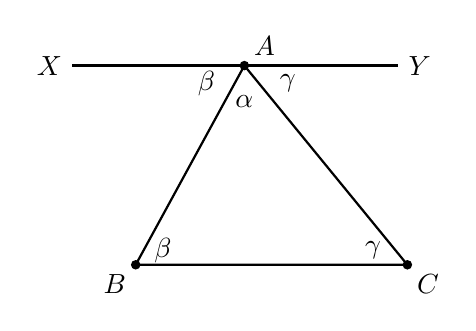
\begin{tikzpicture}[scale=1.15]
  \draw[thick] (0,0)--(3,0)--(1.2,2.2)--cycle;
  \draw[thick] (-0.7,2.2) node[left]{$X$} --(2.9,2.2) node[right]{$Y$};
  \fill (0,0) circle (1.5pt) node[below left]{$B$};
  \fill (3,0) circle (1.5pt) node[below right]{$C$};
  \fill (1.2,2.2) circle (1.5pt) node[above right]{$A$};
  \node at (0.30,0.16) {$\beta$};
  \node at (2.62,0.16) {$\gamma$};
  \node at (0.78,2.00) {$\beta$};
  \node at (1.20,1.80) {$\alpha$};
  \node at (1.68,2.00) {$\gamma$};
\end{tikzpicture}
\end{center}

\noindent
$A$ দিয়ে $BC$-এর সমান্তরাল রেখা $XY$ টানি। $AB$-কে ছেদক ধরলে $\angle XAB$ ও
$\angle ABC$ একান্তর কোণ, তাই $\angle XAB = \beta$। একইভাবে $AC$-কে ছেদক ধরলে
$\angle YAC = \gamma$।

এখন $X$, $A$, $Y$ একই সরলরেখায়, তাই $A$-তে তিনটি কোণ মিলে সরলকোণ:
\[
  \beta + \alpha + \gamma = 180^\circ .
\]
\end{idea}

\begin{idea}[বহিঃস্থ কোণ]
ত্রিভুজের একটি বাহু বাড়ালে যে কোণ তৈরি হয়, তাকে বলে বহিঃস্থ কোণ। $C$-তে বহিঃস্থ
কোণ $= 180^\circ - \gamma$, আর কোণের সমষ্টি থেকে $\alpha + \beta = 180^\circ -
\gamma$। সুতরাং
\[
  \text{বহিঃস্থ কোণ} = \text{দুই অন্তঃস্থ বিপরীত কোণের সমষ্টি}.
\]
এর একটা তাৎক্ষণিক ফল: বহিঃস্থ কোণ দুটি অন্তঃস্থ বিপরীত কোণের যেকোনোটির চেয়ে বড়।
\end{idea}

\begin{idea}[সর্বসমতা বনাম সদৃশতা]
দুটি ত্রিভুজ \textbf{সর্বসম} (congruent, চিহ্ন $\cong$) যদি তাদের অনুরূপ বাহু
সমান এবং অনুরূপ কোণ সমান হয়; অর্থাৎ একটাকে তুলে অন্যটার উপর হুবহু বসানো যায়।

দুটি ত্রিভুজ \textbf{সদৃশ} (similar, চিহ্ন $\sim$) যদি অনুরূপ কোণ সমান হয় এবং
অনুরূপ বাহুগুলো একই অনুপাতে থাকে; অর্থাৎ একটা অন্যটার বড় বা ছোট প্রতিলিপি।

পার্থক্যটা এক কথায়: সর্বসমতা আকার ও আয়তন দুটোই রক্ষা করে, সদৃশতা কেবল আকার।
সর্বসমতা সদৃশতার বিশেষ ক্ষেত্র, যেখানে অনুপাত $1$।

স্বীকার্য ৫ ও ৬ অনুযায়ী কম তথ্য দিয়েই সিদ্ধান্তে পৌঁছানো যায়:
\begin{enumerate}
  \item সর্বসমতা --- SSS (তিন বাহু), SAS (দুই বাহু ও অন্তর্ভুক্ত কোণ),
        ASA (দুই কোণ ও সংলগ্ন বাহু)। (S দিয়ে side, A দিয়ে angle)
  \item সদৃশতা --- AA (দুই কোণ), SAS (দুই বাহুর অনুপাত ও অন্তর্ভুক্ত কোণ),
        SSS (তিন বাহুর অনুপাত)।
\end{enumerate}
\end{idea}

\begin{remark}
তালিকায় SSA নেই, আর এটা ভুলে বাদ পড়েনি। দুটি বাহু ও একটি \emph{অন্তর্ভুক্ত নয়}
এমন কোণ সমান হলেও ত্রিভুজ দুটি ভিন্ন হতে পারে; অর্থাৎ, একই তথ্য থেকে দুটো আলাদা
ত্রিভুজ আঁকা যায়। কোণটি সমকোণ হলে অবশ্য অস্পষ্টতা থাকে না, আর সেই বিশেষ ক্ষেত্রটাই
RHS নামে চেনা।

সদৃশতার তালিকায় আবার AAA আলাদা করে লেখা নেই, কারণ কোণের সমষ্টি $180^\circ$ হওয়ায়
দুটি কোণ মিলে গেলে তৃতীয়টি এমনিতেই মিলে যায়। AA-ই যথেষ্ট।
\end{remark}

\begin{example}
প্রমাণ করো: সমদ্বিবাহু ত্রিভুজের সমান বাহুদ্বয়ের বিপরীত কোণদ্বয় সমান। অর্থাৎ
$\triangle ABC$-এ $AB = AC$ হলে $\angle B = \angle C$।
\end{example}

\begin{solbox}
কৌশলটা প্রথমবার দেখলে চমকে দেয়: আমরা একই ত্রিভুজকে দুবার, দুই ক্রমে গুনব।

$\triangle ABC$ ও $\triangle ACB$ --- এই দুটির তুলনা করি। (দ্বিতীয়টি একই
ত্রিভুজ, শুধু শীর্ষবিন্দুগুলোর নাম অন্য ক্রমে পড়া।)
\begin{enumerate}
  \item $AB = AC$ (দেওয়া আছে);
  \item $\angle BAC = \angle CAB$ (একই কোণ);
  \item $AC = AB$ (একই কথা, উল্টো করে লেখা)।
\end{enumerate}
তাই SAS অনুযায়ী $\triangle ABC \cong \triangle ACB$।

সর্বসম ত্রিভুজে অনুরূপ কোণ সমান। প্রথম তালিকায় $B$-এর অনুরূপ দ্বিতীয় তালিকার
$C$, সুতরাং $\angle B = \angle C$।

মনে খচখচ করলে অন্যভাবেও করা যায়: $\angle A$-এর সমদ্বিখণ্ডক টেনে $BC$-কে $D$-তে
ছেদ করাও, তারপর $\triangle ABD \cong \triangle ACD$ দেখাও SAS দিয়ে। ফল একই।
\end{solbox}

\prob{1} একটি ত্রিভুজের দুটি কোণ $47^\circ$ ও $68^\circ$।
\begin{enumerate}
  \item তৃতীয় কোণটি কত?
  \item তৃতীয় কোণের শীর্ষবিন্দুতে বহিঃস্থ কোণটি কত?
\end{enumerate}

\begin{sol}
\begin{enumerate}
  \item $180^\circ - 47^\circ - 68^\circ = 65^\circ$।
  \item $180^\circ - 65^\circ = 115^\circ$।
\end{enumerate}
যাচাই: বহিঃস্থ কোণ দুই অন্তঃস্থ বিপরীত কোণের সমষ্টি হওয়ার কথা, আর
$47^\circ + 68^\circ = 115^\circ$। মিলেছে।
\end{sol}

\prob{2} $\triangle ABC$-এ $AB = AC$, এবং $\angle A$-এর সমদ্বিখণ্ডক $BC$-কে
$D$ বিন্দুতে ছেদ করে। প্রমাণ করো যে $BD = DC$ এবং $AD \perp BC$।

\begin{sol}
$\triangle ABD$ ও $\triangle ACD$ তুলনা করি:
\begin{enumerate}
  \item $AB = AC$ (দেওয়া আছে);
  \item $\angle BAD = \angle CAD$ ($AD$ সমদ্বিখণ্ডক);
  \item $AD = AD$ (সাধারণ বাহু)।
\end{enumerate}
SAS অনুযায়ী $\triangle ABD \cong \triangle ACD$।

সর্বসমতা থেকে প্রথমেই $BD = DC$।

আবার সর্বসমতা থেকে $\angle ADB = \angle ADC$। কিন্তু $B$, $D$, $C$ একই সরলরেখায়,
তাই এই দুটি কোণ সন্নিহিত সম্পূরক:
\[
  \angle ADB + \angle ADC = 180^\circ .
\]
দুটি সমান কোণের সমষ্টি $180^\circ$ হলে প্রতিটি $90^\circ$। সুতরাং
$AD \perp BC$।

অর্থাৎ সমদ্বিবাহু ত্রিভুজে শীর্ষকোণের সমদ্বিখণ্ডক, ভূমির মধ্যমা আর ভূমির উপর
লম্ব --- তিনটিই একই রেখা। এই তিনটি সাধারণত আলাদা হলেও সমান হয়ে যাওয়াটাই সমদ্বিবাহু
হওয়ার বিশেষত্ব।
\end{sol}

\prob{3} $\triangle ABC$-এ $M$ ও $N$ যথাক্রমে $AB$ ও $AC$ বাহুর মধ্যবিন্দু।
প্রমাণ করো যে $MN \parallel BC$ এবং $MN = \tfrac{1}{2} BC$।

\begin{center}
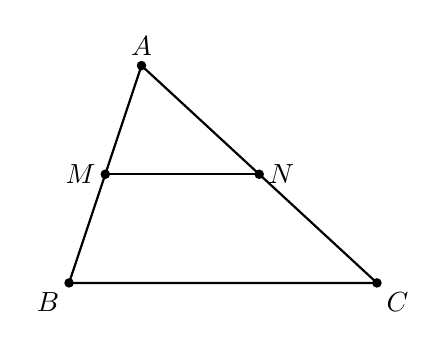
\begin{tikzpicture}[scale=1.15]
  \draw[thick] (0,0)--(3.4,0)--(0.8,2.4)--cycle;
  \draw[thick] (0.4,1.2)--(2.1,1.2);
  \fill (0,0) circle (1.5pt) node[below left]{$B$};
  \fill (3.4,0) circle (1.5pt) node[below right]{$C$};
  \fill (0.8,2.4) circle (1.5pt) node[above]{$A$};
  \fill (0.4,1.2) circle (1.5pt) node[left]{$M$};
  \fill (2.1,1.2) circle (1.5pt) node[right]{$N$};
\end{tikzpicture}
\end{center}

\begin{sol}
$\triangle AMN$ ও $\triangle ABC$ তুলনা করি। $M$ মধ্যবিন্দু হওয়ায়
$AM = \tfrac{1}{2}AB$, এবং $N$ মধ্যবিন্দু হওয়ায় $AN = \tfrac{1}{2}AC$। সুতরাং
\[
  \frac{AM}{AB} = \frac{AN}{AC} = \frac{1}{2},
\]
আর এই দুই জোড়া বাহুর অন্তর্ভুক্ত কোণ $\angle A$ দুই ত্রিভুজে একই।

সদৃশতার SAS শর্ত অনুযায়ী $\triangle AMN \sim \triangle ABC$, অনুপাত $\tfrac{1}{2}$।

সদৃশতা থেকে দুটো জিনিস একসাথে পাই। প্রথমত, তৃতীয় বাহুও একই অনুপাতে:
\[
  MN = \tfrac{1}{2} BC .
\]
দ্বিতীয়ত, অনুরূপ কোণ সমান, তাই $\angle AMN = \angle ABC$। এখন $AB$-কে ছেদক ধরলে
এই দুটি অনুরূপ কোণ, আর তারা সমান। স্বীকার্য ৪-এর বিপরীত অংশ অনুযায়ী
$MN \parallel BC$।

দুটো ফলই এক সদৃশতা থেকে বেরিয়ে এল --- আলাদা করে কিছু করতে হলো না।
\end{sol}

\prob{2} একটি রোদেলা দুপুরে $1.8$ মিটার লম্বা একজন মানুষের ছায়া $2.4$ মিটার।
একই সময়ে পাশের একটি টাওয়ারের ছায়া $30$ মিটার। টাওয়ারটি কত উঁচু? তোমার যুক্তিতে
সদৃশতা কেন খাটছে, সেটাও বলো।

\begin{sol}
সূর্য এত দূরে যে তার রশ্মিগুলোকে সমান্তরাল ধরা যায় --- এটাই মূল অনুমান, এবং
এটা জ্যামিতির কথা নয়, পদার্থবিজ্ঞানের।

মানুষ ও তার ছায়া মিলে একটি ত্রিভুজ, টাওয়ার ও তার ছায়া মিলে আরেকটি। দুটোতেই
মাটির সাথে খাড়া বস্তুর কোণ $90^\circ$। আর সূর্যরশ্মি সমান্তরাল হওয়ায় রশ্মি
মাটির সাথে যে কোণ করে তা দুই জায়গায় সমান (অনুরূপ কোণ)। দুটি কোণ মিলে যাওয়ায়
AA শর্তে ত্রিভুজ দুটি সদৃশ।

সদৃশতা থেকে অনুরূপ বাহুর অনুপাত সমান:
\[
  \frac{h}{30} = \frac{1.8}{2.4} \implies h = 30 \times 0.75 = 22.5 .
\]
টাওয়ারটি $22.5$ মিটার উঁচু।
\end{sol}

\section{থেলিস ও পিথাগোরাস}

\begin{remark}[নাম নিয়ে একটা সতর্কতা]
``থেলিসের উপপাদ্য'' নামে দুটি আলাদা উপপাদ্য প্রচলিত, আর কোন বইয়ে কোনটা বোঝানো
হচ্ছে তা প্রসঙ্গ দেখে বুঝতে হয়। একটি হলো অনুপাত সংক্রান্ত (intercept theorem),
অন্যটি অর্ধবৃত্তস্থ কোণ সংক্রান্ত। দুটোই এখানে আছে, দুটোই প্রমাণসহ। নাম নিয়ে
তর্ক করার কিছু নেই; কোন বিবৃতিটা ব্যবহার করছ, সেটা স্পষ্ট করে বলে দিলেই হলো।
\end{remark}

\begin{idea}[থেলিসের অনুপাত উপপাদ্য]
$\triangle ABC$-এ $BC$-এর সমান্তরাল একটি রেখা $AB$-কে $D$ এবং $AC$-কে $E$
বিন্দুতে ছেদ করলে
\[
  \frac{AD}{AB} = \frac{AE}{AC} .
\]
প্রমাণ: $DE \parallel BC$ হওয়ায় $AB$ ছেদক ধরে $\angle ADE = \angle ABC$
(অনুরূপ কোণ)। আর $\angle A$ দুই ত্রিভুজে সাধারণ। সুতরাং AA শর্তে
$\triangle ADE \sim \triangle ABC$, আর সদৃশ ত্রিভুজে অনুরূপ বাহুর অনুপাত সমান।

সাধারণত যে রূপে দরকার পড়ে সেটা একটু সাজিয়ে পাওয়া যায়। $AB = AD + DB$ ও
$AC = AE + EC$ বসিয়ে সরল করলে দাঁড়ায়
\[
  \frac{AD}{DB} = \frac{AE}{EC} .
\]
\end{idea}

\begin{idea}[বৃত্তের প্রাথমিক কথা]
একটি নির্দিষ্ট বিন্দু $O$ থেকে নির্দিষ্ট দূরত্ব $r$-এ থাকা সব বিন্দুর সমষ্টিই
বৃত্ত। $O$ কেন্দ্র, $r$ ব্যাসার্ধ। এটা একটা সংজ্ঞা, অর্থাৎ চুক্তি। এর
সবচেয়ে বড় ব্যবহার হলো, বৃত্তের উপর যেকোনো দুটি বিন্দু $P$, $Q$ নিলে
$OP = OQ = r$ সঙ্গে সঙ্গে জানা হয়ে যায়। ফলে $\triangle OPQ$ সবসময় সমদ্বিবাহু,
আর আগের অনুচ্ছেদের ফলাফল সরাসরি খাটে।

বৃত্তের দুটি বিন্দুর সংযোজক রেখাংশ হলো জ্যা (chord); কেন্দ্র দিয়ে যাওয়া জ্যা
হলো ব্যাস (diameter), যার দৈর্ঘ্য $2r$।
\end{idea}

\begin{idea}[অর্ধবৃত্তস্থ কোণ এক সমকোণ]
$BC$ একটি ব্যাস এবং $A$ বৃত্তের উপর অন্য যেকোনো বিন্দু হলে $\angle BAC = 90^\circ$।

\begin{center}
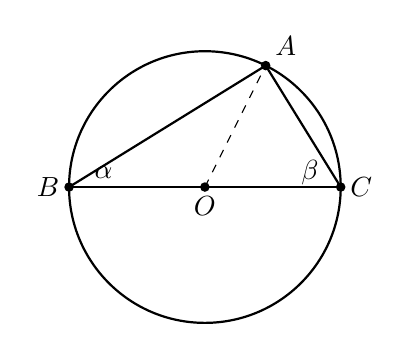
\begin{tikzpicture}[scale=1.15]
  \draw[thick] (0,0) circle (1.5);
  \draw[thick] (-1.5,0)--(1.5,0);
  \coordinate (A) at (63.4:1.5);
  \draw[thick] (-1.5,0)--(A)--(1.5,0);
  \draw[dashed] (0,0)--(A);
  \fill (-1.5,0) circle (1.5pt) node[left]{$B$};
  \fill (1.5,0) circle (1.5pt) node[right]{$C$};
  \fill (0,0) circle (1.5pt) node[below]{$O$};
  \fill (A) circle (1.5pt) node[above right]{$A$};
  \node at (-1.12,0.16) {$\alpha$};
  \node at (1.16,0.16) {$\beta$};
\end{tikzpicture}
\end{center}

\noindent
প্রমাণ: কেন্দ্র $O$ থেকে $A$ পর্যন্ত রেখাংশ টানি। তিনটি রেখাংশ $OA$, $OB$, $OC$
সবই ব্যাসার্ধ, তাই সমান।

$OB = OA$ হওয়ায় $\triangle OAB$ সমদ্বিবাহু, তাই $\angle OBA = \angle OAB$;
ধরি এই মান $\alpha$। একইভাবে $OC = OA$ হওয়ায় $\angle OCA = \angle OAC = \beta$।

এবার $\triangle ABC$-এর তিন কোণ যোগ করি। $B$-তে কোণ $\alpha$, $C$-তে কোণ
$\beta$, আর $A$-তে কোণ $\alpha + \beta$ (কারণ $OA$ রশ্মিটি $\angle BAC$-কে
দু-ভাগ করেছে)। সুতরাং
\[
  \alpha + \beta + (\alpha + \beta) = 180^\circ \implies
  2(\alpha + \beta) = 180^\circ \implies \alpha + \beta = 90^\circ .
\]
আর $\angle BAC = \alpha + \beta = 90^\circ$।

লক্ষ করো, $A$ কোথায় আছে তা নিয়ে প্রমাণে একটি শব্দও খরচ হয়নি --- ব্যাসের এক পাশে
যেকোনো জায়গায় থাকলেই চলবে। এটাই ফলাফলটাকে অবাক করার মতো করে তোলে।
\end{idea}

\begin{idea}[পিথাগোরাসের উপপাদ্য]
$\triangle ABC$-এ $\angle A = 90^\circ$ হলে $AB^2 + AC^2 = BC^2$।

\begin{center}
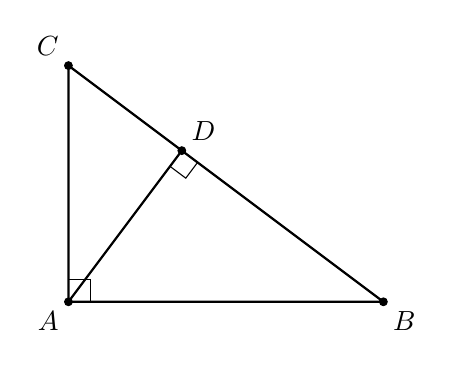
\begin{tikzpicture}[scale=1.0]
  \draw[thick] (0,0)--(4,0)--(0,3)--cycle;
  \draw[thick] (0,0)--(1.44,1.92);
  \draw (0,0.28)--(0.28,0.28)--(0.28,0);
  \draw (1.29,1.72)--(1.49,1.57)--(1.64,1.77);
  \fill (0,0) circle (1.6pt) node[below left]{$A$};
  \fill (4,0) circle (1.6pt) node[below right]{$B$};
  \fill (0,3) circle (1.6pt) node[above left]{$C$};
  \fill (1.44,1.92) circle (1.6pt) node[above right]{$D$};
\end{tikzpicture}
\end{center}

\noindent
প্রমাণ: $A$ থেকে অতিভুজ $BC$-এর উপর লম্ব $AD$ টানি।

$\triangle DBA$ ও $\triangle ABC$ তুলনা করি। $\angle B$ দুটিতেই একই, আর
$\angle BDA = \angle BAC = 90^\circ$। AA শর্তে $\triangle DBA \sim \triangle ABC$।
অনুরূপ বাহুর অনুপাত সমান হওয়ায়
\[
  \frac{BD}{AB} = \frac{AB}{BC} \implies AB^2 = BC \cdot BD .
\]
ঠিক একইভাবে $\triangle DAC \sim \triangle ABC$ ($\angle C$ সাধারণ, দুটিতেই একটি
সমকোণ), যা দেয়
\[
  AC^2 = BC \cdot CD .
\]
দুটি যোগ করি, আর $D$ যেহেতু $B$ ও $C$-এর মাঝে, তাই $BD + CD = BC$:
\[
  AB^2 + AC^2 = BC(BD + CD) = BC \cdot BC = BC^2 .
\]
\end{idea}

\begin{example}
একটি বৃত্তের ব্যাস $BC = 26$ সেমি, এবং $A$ বৃত্তের উপর একটি বিন্দু যেখানে
$AB = 10$ সেমি। $AC$ নির্ণয় করো।
\end{example}

\begin{solbox}
$BC$ ব্যাস এবং $A$ বৃত্তের উপর, তাই অর্ধবৃত্তস্থ কোণ উপপাদ্য অনুযায়ী
$\angle BAC = 90^\circ$। এখন পিথাগোরাস খাটে:
\[
  AB^2 + AC^2 = BC^2 \implies 100 + AC^2 = 676 \implies AC^2 = 576 .
\]
স্বীকার্য ৮ অনুযায়ী $576$-এর একটিমাত্র অঋণাত্মক বর্গমূল আছে, আর দৈর্ঘ্য
অঋণাত্মক, তাই $AC = 24$ সেমি।

দুটো আলাদা উপপাদ্য পরপর লাগল --- প্রথমটা সমকোণটা \emph{খুঁজে দিল}, দ্বিতীয়টা
সেই সমকোণকে \emph{ব্যবহার করল}। এই জোড়াটা বৃত্ত ও সমকোণের সমস্যায় বারবার আসবে।
\end{solbox}

\prob{2} $BC$ ব্যাসবিশিষ্ট একটি বৃত্তের উপর $A$ একটি বিন্দু, যেখানে $AB = 16$
সেমি ও $AC = 30$ সেমি।
\begin{enumerate}
  \item বৃত্তটির ব্যাসার্ধ কত?
  \item কেন্দ্র থেকে $A$ বিন্দুর দূরত্ব কত? (হিসাব না করে উত্তর দেওয়া যায় ---
        কেন?)
\end{enumerate}

\begin{sol}
\begin{enumerate}
  \item $\angle BAC = 90^\circ$ (অর্ধবৃত্তস্থ কোণ), তাই
        \[
          BC^2 = 16^2 + 30^2 = 256 + 900 = 1156 \implies BC = 34 .
        \]
        ব্যাস $34$ সেমি, তাই ব্যাসার্ধ $17$ সেমি।
  \item $A$ বৃত্তের উপর একটি বিন্দু, আর কেন্দ্র থেকে বৃত্তের যেকোনো বিন্দুর
        দূরত্বই ব্যাসার্ধ --- এটাই বৃত্তের সংজ্ঞা। সুতরাং দূরত্ব $17$ সেমি,
        কোনো হিসাব ছাড়াই।
\end{enumerate}
এখানেই সংজ্ঞাকে চুক্তি হিসেবে দেখার লাভ। ``বৃত্ত'' শব্দটা মেনে নেওয়া মানেই
$OA = r$ মেনে নেওয়া; আলাদা করে প্রমাণের কিছু নেই।
\end{sol}

\prob{2} একটি আয়তাকার মাঠের দৈর্ঘ্য $45$ মিটার ও প্রস্থ $24$ মিটার। এক কোণ থেকে
বিপরীত কোণে যেতে কেউ যদি দুই বাহু ধরে হাঁটার বদলে কর্ণ বরাবর হাঁটে, তবে কত মিটার
কম হাঁটতে হবে?

\begin{sol}
আয়তক্ষেত্রের কোণগুলো সমকোণ, তাই কর্ণ $d$-এর জন্য পিথাগোরাস খাটে:
\[
  d^2 = 45^2 + 24^2 = 2025 + 576 = 2601 \implies d = 51 .
\]
($51^2 = 2601$ --- যাচাই করে নাও।)

দুই বাহু ধরে হাঁটলে দূরত্ব $45 + 24 = 69$ মিটার। সুতরাং সাশ্রয়
\[
  69 - 51 = 18 \text{ মিটার}.
\]
\end{sol}

\prob{3} পিথাগোরাসের উপপাদ্যের বিপরীতটি প্রমাণ করো: $\triangle ABC$-এ যদি
$AB^2 + AC^2 = BC^2$ হয়, তবে $\angle A = 90^\circ$।

\begin{sol}
সরাসরি প্রমাণের চেষ্টা এখানে আটকে যায়, কারণ হাতে কেবল বাহুর দৈর্ঘ্য আছে, কোনো
কোণ নেই। তাই কৌশল হলো একটা \emph{নতুন} ত্রিভুজ বানানো, যার সমকোণ থাকার কথা আমরা
জানি।

ধরি $AB = c$, $AC = b$, $BC = a$, এবং দেওয়া আছে $b^2 + c^2 = a^2$।

এখন $\triangle DEF$ আঁকি যার $\angle F = 90^\circ$, $DF = b$ এবং $EF = c$।
(এমন ত্রিভুজ আঁকা যায় : $F$-এ একটি সমকোণ নিয়ে দুই বাহুতে $b$ ও $c$ মেপে
নিলেই হলো।) এই ত্রিভুজে পিথাগোরাস খাটে, কারণ সেখানে সমকোণ আছে:
\[
  DE^2 = DF^2 + EF^2 = b^2 + c^2 = a^2 .
\]
$DE$ ও $a$ দুটোই অঋণাত্মক এবং তাদের বর্গ সমান; স্বীকার্য ৮ অনুযায়ী অঋণাত্মক
বর্গমূল একটিমাত্র, তাই $DE = a$।

এবার $\triangle ABC$ ও $\triangle EFD$ তুলনা করি: $BC = EF$ $AB = c = EF$, $AC = b = DF$, $BC = a = DE$। তিন জোড়া বাহুই সমান, তাই
SSS অনুযায়ী $\triangle ABC \cong \triangle EFD$।

সর্বসমতা থেকে অনুরূপ কোণ সমান। $A$-এর অনুরূপ হলো $F$, সুতরাং
$\angle A = \angle F = 90^\circ$।

এই কৌশলটার নাম নেই, কিন্তু ধরনটা চিনে রাখো: যা প্রমাণ করতে চাই তা \emph{ধরে
নিয়ে} একটা আদর্শ বস্তু বানাও, তারপর দেখাও মূল বস্তুটা তার সাথে সর্বসম।
\end{sol}

\section{ক্ষেত্রফল ও পরিসীমা}

\begin{idea}[ক্ষেত্রফল যোগাত্মক]
পরিসীমা মানে সীমানার মোট দৈর্ঘ্য : বহুভুজের ক্ষেত্রে কেবল বাহুগুলো যোগ করা।
ক্ষেত্রফল তার চেয়ে সূক্ষ্ম, কারণ ``ভেতরের পরিমাণ'' মাপার জন্য একটা একক লাগে।
স্বীকার্য ৭ সেই একক ঠিক করে দেয়: আয়তক্ষেত্রের ক্ষেত্রফল দৈর্ঘ্য গুণ প্রস্থ।

সবচেয়ে বেশি কাজে লাগে যোগাত্মকতা: একটি চিত্রকে পৃথক পৃথক (non-overlapping) কয়েকটি টুকরায়
ভাগ করলে টুকরাগুলোর ক্ষেত্রফলের সমষ্টিই মূল ক্ষেত্রফল। এই একটা কথা থেকেই
বাকি সব সূত্র বেরোয়।
\end{idea}

\begin{idea}[ত্রিভুজের ক্ষেত্রফল]
প্রথমে সমকোণী ত্রিভুজ। লম্ব বাহু $p$ ও $q$ বিশিষ্ট একটি সমকোণী ত্রিভুজের একটা
সর্বসম প্রতিলিপি নিয়ে অতিভুজ বরাবর উল্টে জুড়ে দিলে $p \times q$ মাপের একটি
আয়তক্ষেত্র পাওয়া যায়। দুটি টুকরার ক্ষেত্রফল সমান (সর্বসম) এবং যোগাত্মকতা অনুযায়ী
তাদের যোগফল $pq$, তাই প্রতিটির ক্ষেত্রফল $\tfrac{1}{2}pq$।

এবার যেকোনো ত্রিভুজ। ভূমি $b$-এর উপর শীর্ষবিন্দু থেকে লম্ব (উচ্চতা) $h$ টানি।
লম্বের পাদবিন্দু ভূমির ভেতরে পড়লে ত্রিভুজটি দুটি সমকোণী ত্রিভুজে ভাগ হয়ে যায়,
যাদের ভূমি $b_1$ ও $b_2$ এবং $b_1 + b_2 = b$। যোগাত্মকতা অনুযায়ী
\[
  \text{ক্ষেত্রফল} = \tfrac{1}{2}b_1 h + \tfrac{1}{2}b_2 h
  = \tfrac{1}{2}(b_1 + b_2)h = \tfrac{1}{2}bh .
\]
পাদবিন্দু ভূমির বাইরে পড়লে (স্থূলকোণী ত্রিভুজে যা ঘটে) একই হিসাব চলে, শুধু যোগের
বদলে বিয়োগ; বড় সমকোণী ত্রিভুজ থেকে বাড়তি টুকরাটা বাদ দিতে হয়। ফল একই।
\end{idea}

\begin{idea}[$\pi$ কোথা থেকে আসে]
$\pi$ কোনো আকাশ থেকে পড়া সংখ্যা নয়, এবং $22/7$ তার মান নয়; ওটা কেবল একটা
সুবিধাজনক আসন্ন মান।

আসল কথাটা হলো: সব বৃত্ত পরস্পর সদৃশ। যেকোনো দুটি বৃত্ত নিলে একটাকে বড় বা ছোট
করে হুবহু অন্যটা বানানো যায়, কারণ বৃত্তের আকার নির্ধারণে ব্যাসার্ধ ছাড়া আর কোনো
তথ্যই নেই। সদৃশ চিত্রে সব দৈর্ঘ্য একই অনুপাতে বাড়ে-কমে, তাই পরিধি ও ব্যাসের
অনুপাত \emph{সব} বৃত্তের জন্য একই সংখ্যা হতে বাধ্য।

সেই সাধারণ সংখ্যাটার নামই $\pi$। অর্থাৎ $\pi$-এর সংজ্ঞা
\[
  \pi = \frac{\text{পরিধি}}{\text{ব্যাস}}, \qquad\text{সুতরাং}\qquad C = 2\pi r .
\]
এটা প্রমাণ নয়, সংজ্ঞা --- প্রমাণটুকু হলো অনুপাতটা যে ধ্রুব, সেটুকু।
\end{idea}

\begin{remark}[বৃত্তের ক্ষেত্রফল --- একটা যুক্তি, প্রমাণ নয়]
বৃত্তকে কেন্দ্র থেকে $n$টি সরু বৃত্তকলায় কাটো, তারপর কলাগুলো একটার পাশে আরেকটা
উল্টো-সোজা করে সাজাও। যত বেশি টুকরা করবে, সাজানো আকৃতিটা তত বেশি একটা
আয়তক্ষেত্রের মতো দেখাবে, যার ভূমি পরিধির অর্ধেক অর্থাৎ $\pi r$ এবং উচ্চতা $r$।
তাই ক্ষেত্রফল $\pi r \cdot r = \pi r^2$।

এটা \emph{প্রমাণ নয়}, আর সেটা স্পষ্ট করে বলা দরকার। ``যত বেশি টুকরা, তত বেশি
আয়তক্ষেত্রের মতো'' কথাটার কোনো নির্ভুল অর্থ এখনো আমাদের হাতে নেই; সেই অর্থটার
নাম limit, আর সেটা আসছে অধ্যায় ১৪-এ। ততক্ষণ $A = \pi r^2$ সূত্রটা ব্যবহার করব।

আর হ্যাঁ, $\pi$ অমূলদ : কোনো ভগ্নাংশ দিয়েই একে হুবহু লেখা যায় না। প্রমাণটা
কঠিন এবং এই সিরিজের বাইরে, কিন্তু ফলটা জেনে রাখা ভালো, কারণ এর মানে $22/7$ বা
$3.1416$ লিখলে সবসময়ই কিছুটা ভুল থেকেই যাচ্ছে।
\end{remark}

\begin{example}
একটি বৃত্তের ব্যাসার্ধ $7$ সেমি। একই পরিসীমার একটি বর্গক্ষেত্র নিলে কার ক্ষেত্রফল
বেশি? ($\pi \approx 22/7$ ধরো।)
\end{example}

\begin{solbox}
বৃত্তের পরিধি
\[
  C = 2\pi r \approx 2 \times \frac{22}{7} \times 7 = 44 \text{ সেমি}.
\]
একই পরিসীমার বর্গক্ষেত্রের বাহু $44/4 = 11$ সেমি, তাই তার ক্ষেত্রফল
$11^2 = 121$ বর্গসেমি।

বৃত্তের ক্ষেত্রফল
\[
  A = \pi r^2 \approx \frac{22}{7} \times 49 = 154 \text{ বর্গসেমি}.
\]

বৃত্তের ক্ষেত্রফল বেশি, প্রায় $27\%$ বেশি।

শিক্ষণীয় কথাটা এই; পরিসীমা দিয়ে ক্ষেত্রফল নির্ধারিত হয় না। একই দৈর্ঘ্যের
দড়ি দিয়ে ঘেরা বিভিন্ন আকৃতির ক্ষেত্রফল বিভিন্ন, আর তার মধ্যে বৃত্তেরটাই সবচেয়ে
বড়। এই শেষ দাবিটা প্রমাণ করা কঠিন, তাই এখানে কেবল একটা উদাহরণ দেখলাম, প্রমাণ নয়।
\end{solbox}

\prob{2} প্রমাণ করো যে যেকোনো ত্রিভুজে প্রতিটি বাহু ও তার অনুরূপ উচ্চতার গুণফল
সমান। অর্থাৎ বাহু $a, b, c$ এবং তাদের উপর উচ্চতা যথাক্রমে $h_a, h_b, h_c$ হলে
\[
  a\,h_a = b\,h_b = c\,h_c .
\]

\begin{sol}
ত্রিভুজটির ক্ষেত্রফলকে $S$ ধরি। ক্ষেত্রফল ত্রিভুজের একটা ধর্ম; কোন বাহুকে
ভূমি ধরলাম তার উপর নির্ভর করে না। কিন্তু তিনটি বাহুর যেকোনোটিকে ভূমি ধরেই
হিসাব করা যায়:
\[
  S = \tfrac{1}{2} a h_a, \qquad S = \tfrac{1}{2} b h_b, \qquad
  S = \tfrac{1}{2} c h_c .
\]
তিনটিই একই সংখ্যা $S$-এর সমান, তাই তারা পরস্পর সমান। দুই দিয়ে গুণ করলে
\[
  a h_a = b h_b = c h_c = 2S .
\]

একটা কাজে লাগার ফল: বাহু বড় হলে তার উচ্চতা ছোট হতে বাধ্য, কারণ গুণফল ধ্রুব।
\end{sol}

\prob{3} $\triangle ABC$-এর $BC$ বাহুর উপর $D$ একটি বিন্দু। প্রমাণ করো যে
\[
  \frac{\triangle ABD\text{-এর ক্ষেত্রফল}}{\triangle ADC\text{-এর ক্ষেত্রফল}}
  = \frac{BD}{DC} .
\]

\begin{center}
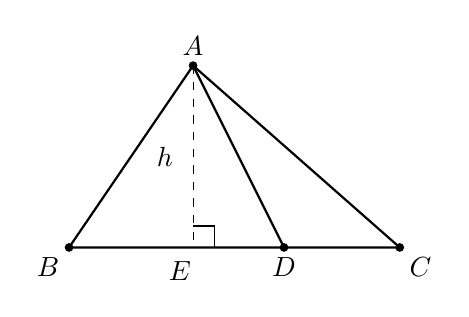
\begin{tikzpicture}[scale=1.05]
  \draw[thick] (0,0)--(4,0)--(1.5,2.2)--cycle;
  \draw[thick] (1.5,2.2)--(2.6,0);
  \draw[dashed] (1.5,2.2)--(1.5,0);
  \draw (1.5,0.26)--(1.76,0.26)--(1.76,0);
  \fill (0,0) circle (1.5pt) node[below left]{$B$};
  \fill (4,0) circle (1.5pt) node[below right]{$C$};
  \fill (1.5,2.2) circle (1.5pt) node[above]{$A$};
  \fill (2.6,0) circle (1.5pt) node[below]{$D$};
  \node at (1.34,-0.28) {$E$};
  \node at (1.16,1.10) {$h$};
\end{tikzpicture}
\end{center}

\begin{sol}
মূল পর্যবেক্ষণ: $A$ থেকে $BC$ রেখার উপর লম্ব $AE = h$ টানলে সেই একই লম্বটি
$\triangle ABD$ ও $\triangle ADC$ --- দুটোরই উচ্চতা, কারণ $B$, $D$, $C$ তিনটি
বিন্দুই একই সরলরেখায় এবং তিনটি ত্রিভুজেরই শীর্ষবিন্দু $A$।

তাই $BD$-কে ভূমি ধরে
\[
  \triangle ABD\text{-এর ক্ষেত্রফল} = \tfrac{1}{2} \cdot BD \cdot h,
\]
আর $DC$-কে ভূমি ধরে
\[
  \triangle ADC\text{-এর ক্ষেত্রফল} = \tfrac{1}{2} \cdot DC \cdot h .
\]
ভাগ করলে $\tfrac{1}{2}$ ও $h$ কেটে যায়:
\[
  \frac{\tfrac{1}{2}\, BD\, h}{\tfrac{1}{2}\, DC\, h} = \frac{BD}{DC} .
\]

যাচাই হিসেবে যোগাত্মকতা মিলিয়ে দেখো: দুটি ক্ষেত্রফল যোগ করলে
$\tfrac{1}{2}(BD + DC)h = \tfrac{1}{2} BC \cdot h$, যা $\triangle ABC$-এর
ক্ষেত্রফল। মিলেছে।

বিশেষ ক্ষেত্র হিসেবে $D$ যদি $BC$-এর মধ্যবিন্দু হয়, তবে অনুপাত $1$  অর্থাৎ
মধ্যমা ত্রিভুজকে সমান ক্ষেত্রফলের দুই ভাগে ভাগ করে। মধ্যমা কিন্তু ত্রিভুজটাকে
দুটি সর্বসম ত্রিভুজে ভাগ করে না; কেবল ক্ষেত্রফল সমান করে। এই পার্থক্যটা খেয়াল
রেখো।
\end{sol}

\end{document}
